% Generated from the public primitive catalog. Original Atlas drawing; Apache-2.0.
% Target: aria-128; view: detail
\documentclass[border=9pt]{standalone}
% Original Atlas figure theme. Apache-2.0; see the repository LICENSE.
\usepackage[T1]{fontenc}
\usepackage{lmodern}
\usepackage{amsmath,amssymb}
\usepackage{tikz}
\usetikzlibrary{arrows.meta,positioning,calc,fit,backgrounds,decorations.pathreplacing,matrix}
\definecolor{atlasInk}{HTML}{172235}
\definecolor{atlasTeal}{HTML}{0D7B7D}
\definecolor{atlasMuted}{HTML}{637278}
\definecolor{atlasFill}{HTML}{EAF4F2}
\definecolor{atlasLine}{HTML}{B6C8C7}
\tikzset{
  every picture/.style={line width=.65pt,draw=atlasInk,>=Latex},
  every node/.style={text=atlasInk,font=\sffamily\small},
  box/.style={draw,rounded corners=1.5pt,minimum height=.9cm,minimum width=1.6cm,align=center,inner sep=6pt,fill=white},
  accent/.style={box,draw=atlasTeal,fill=atlasFill},
  wire/.style={->,line width=.7pt},
  keywire/.style={wire,draw=atlasTeal,dashed},
  xor/.style={draw,circle,fill=white,inner sep=0pt,minimum size=.38cm},
  add/.style={draw,rectangle,fill=white,inner sep=0pt,minimum size=.38cm},
  note/.style={font=\sffamily\scriptsize,text=atlasMuted,align=center},
  phase/.style={font=\sffamily\small\bfseries,text=atlasTeal},
  group/.style={draw=atlasLine,dashed,rounded corners=2pt,inner sep=8pt}
}
\newcommand{\rotl}{\mathbin{\lll}}
\newcommand{\rotr}{\mathbin{\ggg}}
\newcommand{\kx}{\operatorname{Keccak}\!\text{-}\!f[1600]}

\newcommand{\AtlasKeyBits}{128}
\newcommand{\AtlasKeyWords}{4}
\newcommand{\AtlasRounds}{12}
\newcommand{\AtlasPriorRounds}{11}
\newcommand{\AtlasRoundKeys}{13}
\newcommand{\AtlasDoubleRounds}{6}
\newcommand{\AtlasSixRoundGroups}{2}
\newcommand{\AtlasFLGroups}{1}
\newcommand{\AtlasRoundStart}{12}
\newcommand{\AtlasBlockBits}{128}
\newcommand{\AtlasOutputBits}{d}
\newcommand{\AtlasStateBits}{8w}
\newcommand{\AtlasNonceBits}{v}
\newcommand{\AtlasCounterBits}{q}
\newcommand{\AtlasStreamBlockBits}{b}
\newcommand{\AtlasRate}{r}
\newcommand{\AtlasCapacity}{c}
\newcommand{\AtlasSteps}{N}
\newcommand{\AtlasLastStep}{N-1}
\newcommand{\AtlasWordBits}{w}
\newcommand{\AtlasHashWords}{h}
\newcommand{\AtlasFeedForward}{\boxplus}
\newcommand{\AtlasByteOrder}{big-endian}
\newcommand{\AtlasDomain}{01}
\newif\ifAtlasXof
\AtlasXoffalse
\begin{document}
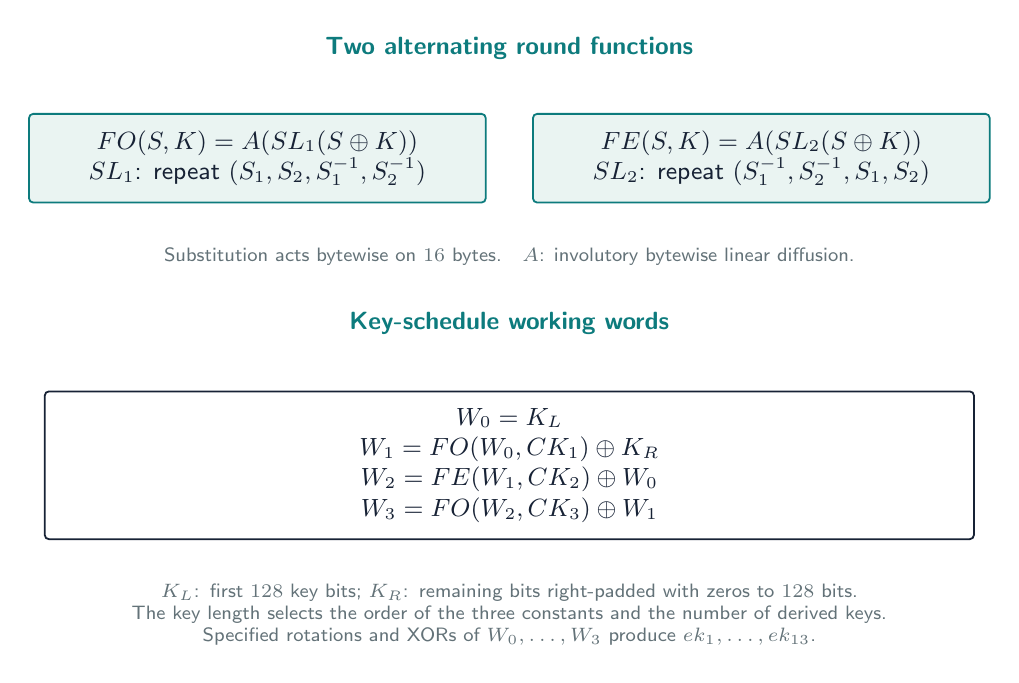
\begin{tikzpicture}
  \node[phase] at (6,3.1) {Two alternating round functions};
  \node[accent,minimum width=5.8cm] at (2.8,1.7) {$FO(S,K)=A(SL_1(S\oplus K))$\\$SL_1$: repeat $(S_1,S_2,S_1^{-1},S_2^{-1})$};
  \node[accent,minimum width=5.8cm] at (9.2,1.7) {$FE(S,K)=A(SL_2(S\oplus K))$\\$SL_2$: repeat $(S_1^{-1},S_2^{-1},S_1,S_2)$};
  \node[note] at (6,.45) {Substitution acts bytewise on $16$ bytes.\quad $A$: involutory bytewise linear diffusion.};
  \node[phase] at (6,-.4) {Key-schedule working words};
  \node[box,minimum width=11.8cm] at (6,-2.2) {$W_0=K_L$\\$W_1=FO(W_0,CK_1)\oplus K_R$\\$W_2=FE(W_1,CK_2)\oplus W_0$\\$W_3=FO(W_2,CK_3)\oplus W_1$};
  \node[note,text width=12cm] at (6,-4.1) {$K_L$: first $128$ key bits; $K_R$: remaining bits right-padded with zeros to $128$ bits.\\The key length selects the order of the three constants and the number of derived keys.\\Specified rotations and XORs of $W_0,\ldots,W_3$ produce $ek_1,\ldots,ek_{\AtlasRoundKeys}$.};
\end{tikzpicture}

\end{document}
